\section{Results and discussion}
\subsection{Optimisation of the classifier parameters}
By performing a five fold cross validation during the training stage the most
optimal parameter set for the RF algorithm were discovered. It was found that
for all levels except the first, a value of 5 yields optimal results for the
minimum samples per leaf parameter. For level 1, this optimal value was
significantly higher at 55. This makes sense as higher values correspond to less
complex classifiers.

The accuracy that was reached was respectively 80,5\%, 97,9\%, 98,1\% and 98,2\%
for the four consecutive levels. This shows that the first two levels in the
cascade contributed more in the process of removing negative voxels the the two
last levels. The latter however were not useless as they still increased the
level of accuracy. The fourth level for example still eliminated about 600
voxels per scan. Though, as mentioned before, the accuracy metric should be taken
with a grain of salt in highly unbalanced classification tasks.

For each level of the classifier, a threshold was set to determine which voxels
would be allowed to the next level (i.e. which voxels showed a higher nodule
probability). In order to avoid discarding nodule voxels of small nodules a
rather low threshold had to be set. These were empirically determined at 20\%,
40\%, 40\% and 70\% for the four levels respectively, although more rigorous
testing might yield even better values.

\subsection{Validation results}
In this section, we will illustrate our results based on two slices from the
fiftieth LIDC dataset. The volume dimensions are $512 \times 512\times 139$ and
it contains one nodule around slice 95. As figure \ref{fig:d50} shows, slice 50
contains no nodules while slice 95 indeed contains exactly one. After applying
the lung mask, 13,59\% of all voxels remain.

\begin{figure}[ht]
\begin{center}
	\begin{subfigure}[b]{\linewidth}
		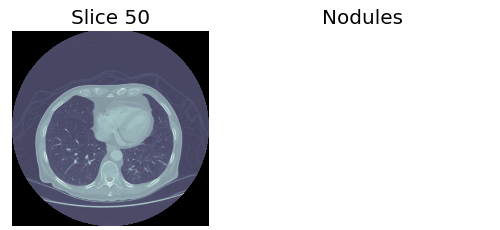
\includegraphics[width=\linewidth]{img/cascades/D50S50.png}
		\caption{Slice 50}
	\end{subfigure}
	\begin{subfigure}[b]{\linewidth}
		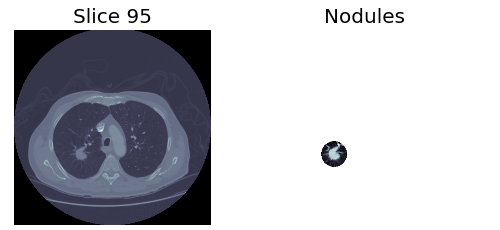
\includegraphics[width=\linewidth]{img/cascades/D50S95.png}
  		\caption{Slice 95}
	\end{subfigure}
	\caption{Example of two slices in dataset 50, one without and one with a
	nodule.}
	\label{fig:d50}
\end{center}
\end{figure}

\paragraph{Level 1}
As expected, we get a significant reduction in the number of voxels. More
specifically only soft tissue structures -- i.e. lung wall, bronchi/bronchioli
and nodules -- remain. The threshold performs a straightforward segmentation and
can not be improved much.

\begin{figure}[p]
\begin{center}
	\begin{subfigure}[b]{\linewidth}
		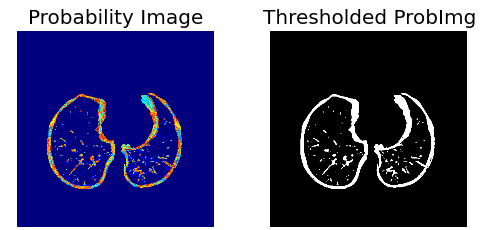
\includegraphics[width=\linewidth]{img/cascades/D50S50L1.png}
		\caption{Level 1 -- Threshold: 20\% -- 5,74\% remaining}
	\end{subfigure}
	\begin{subfigure}[b]{\linewidth}
		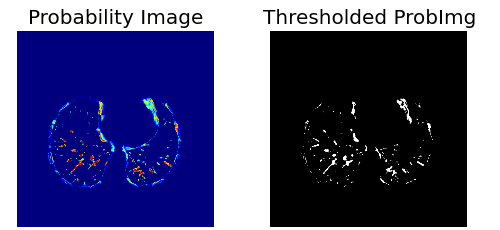
\includegraphics[width=\linewidth]{img/cascades/D50S50L2.png}
		\caption{Level 2 -- Threshold: 40\% -- 1,86\% remaining}
	\end{subfigure}
	\begin{subfigure}[b]{\linewidth}
		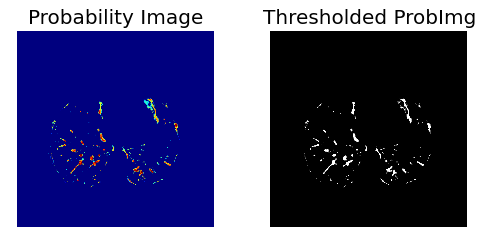
\includegraphics[width=\linewidth]{img/cascades/D50S50L3.png}
		\caption{Level 3 -- Threshold: 40\% -- 1,55\% remaining}
	\end{subfigure}
	\begin{subfigure}[b]{\linewidth}
		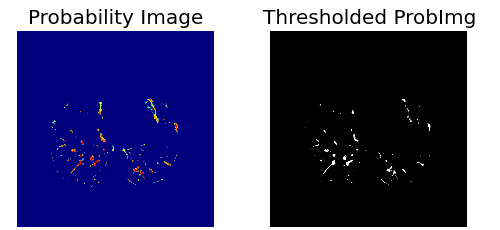
\includegraphics[width=\linewidth]{img/cascades/D50S50L4.png}
		\caption{Level 4 -- Threshold: 70\% -- 0,54\% remaining}
	\end{subfigure}
  \caption{Processed versions of slice 50 in dataset 50. Left: probability
  image. Right: threshold of probability image showing the voxels that continue
  to the next level in the cascade. The algorithm started with 13,59\% of all 
  voxels remaining after lung segmentation.}
  \label{fig:d50s50}
\end{center}
\end{figure}

\begin{figure}[p]
\begin{center}
	\begin{subfigure}[b]{\linewidth}
		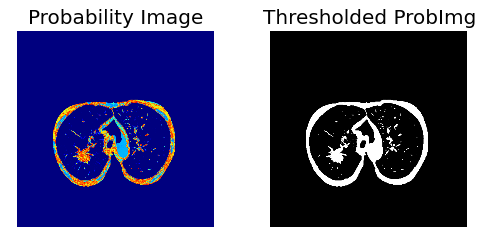
\includegraphics[width=\linewidth]{img/cascades/D50S95L1.png}
		\caption{Level 1}
	\end{subfigure}
	\begin{subfigure}[b]{\linewidth}
		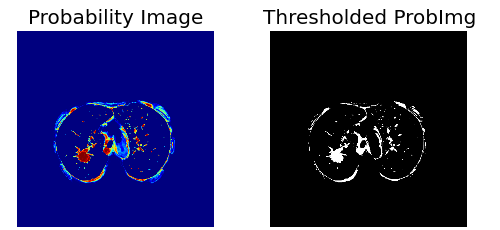
\includegraphics[width=\linewidth]{img/cascades/D50S95L2.png}
		\caption{Level 2}
	\end{subfigure}
	\begin{subfigure}[b]{\linewidth}
		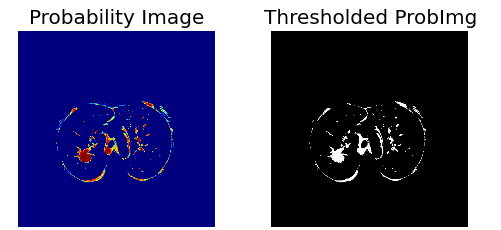
\includegraphics[width=\linewidth]{img/cascades/D50S95L3.png}
		\caption{Level 3}
	\end{subfigure}
	\begin{subfigure}[b]{\linewidth}
		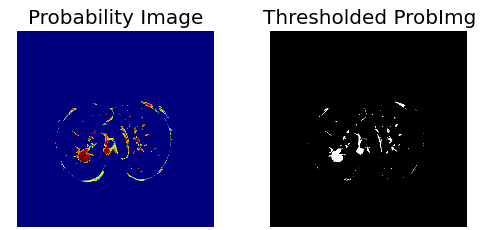
\includegraphics[width=\linewidth]{img/cascades/D50S95L4.png}
		\caption{Level 4}
	\end{subfigure}
  \caption{Processed versions of slice 95 in dataset 50. Left: probability
  image. Right: threshold of probability image showing the voxels that continue
  to the next level in the cascade. The same thresholds and remaining counts
  apply as in figure \ref{fig:d50s50}.}
  \label{fig:d50s95}
\end{center}
\end{figure}

\paragraph{Level 2}
This level was meant to highlight nodule-sized blobs while reducing the response
of other structures, in particular lung walls. The laplacian filter certainly
succeeded in the former, although we still get a medium-high response from
certain wall segments at times. Unfortunately, the laplacian also highlights the
smaller structures in the lung. This was inevitable as we needed LoG filters
with small sigmas to find small nodules. There is definitely room for
improvement in threshold level. A higher threshold could discard more wall
voxels while retaining nodules. In conclusion it is still a well performing
feature that significantly reduces the voxel count, although it has some
unfortunate side effects.

\paragraph{Level 3 and 4}
The goal here was to discriminate between small bronchioli and blood vessels on
the one hand, and small nodules on the other hand by means of 3D averaging.
Unfortunately, this feature does not perform as well as hoped: there is only a
margin decrease in non-nodule voxels. Note that the fourth level feature with
the larger internal threshold works slightly better, but still not satisfactory.
Future work should either fine-tune the parameters of this method or find a more
effective method altogether.

The obtained sensitivity of the algorithm was 100,00\% with an average of 2,17
TP and 4279,43 FP per scan. This high number of FP results a in very low
precision of 0,0634\%. Training the algorithm on 30 scans took 1 hour and 50
minutes. The processing of a new medium large dataset (136 slices) takes about
10 minutes.

Keeping in mind that comparing different studies is difficult (see section
\ref{sec:performance}), some relevant results from literature are presented
here. \cite{teramoto} used a cylindrical nodule-enhancement filter and performed
a FP reduction using a SVM classifier. This method reached a sensitivity of 80\%
and 4,2 FP per LIDC/IDRI scan. The detection speed was 25-34 seconds per scan.
\cite{elbaz} applied template matching and found a sensitivity of 82,3\% and a
specificity of 9,2\%. The time to process 1 scan in C++ was about 5 minutes.
\cite{lee2010} tested an ensemble classification aided by clustering (CAC)
method on a set of nodules and non-nodule examples and they obtained a
classification accuracy of 97,72\%. An execution time of 190 seconds was
registered.

These results indicate our algorithm performed well concerning detecting all
nodules, but the amount of FP has to be reduced to get the precision up. At the
moment, the algorithm is simply not strict enough: it detects all nodules but at
a high FP cost. This amount can be reduced in a first stage by determining
the optimal value for all parameters, such as the threshold for each cascade
level.

Our ``potential nodule'' clustering strategy also plays a significant role here.
By clustering individual voxels together we hope to make them more comparable
to nodules, but this is not always the case. Some clusters are simply too small
to even represent a realistic nodule. Filtering out these clusters will help
boost our results.

Another way of improving the algorithm is increasing the amount of training
data. To determine the optimal amount of datasets a trade-off should be made
between the time it takes to train the algorithm with extra datasets and the
diminishing marginal improvements in the performances of that action. 

A third possibility is implementing more features (e.g. haar features),
especially features focusing on removing edges and eliminating the bronchioles.
On the other hand, implementing more features will increase the processing time.
However, by optimising the thresholds in the existing algorithm these things can
also be (partially) achieved. The threshold on level can be set higher which
will remove more edges. For eliminating the bronchioles the parameters of the 3D
averaging features should be optimised. The results from the literature also
show that we have a long processing time. However, one has to take into account
that the implementation of this algorithm was done in Python -- an interpreted
language -- which makes it inherently slower than low-level compiled languages
such as C++. Nevertheless, Python was chosen for its rapid prototyping
abilities. Future work may implement our algorithm in C++ or another compiled
language to speed up the computational process.

\cite{ginneken} compared the performances of six nodule detection CAD algorithms
on the same validation dataset. The sensitivities at seven levels of false
positive detection were calculated and then averaged. The best performing method
in this study yielded an average sensitivity of 63,2\% for the detection of all
kinds of nodules. The sensitivity per nodule type was also provided: small
nodules (63,4\%), large nodules (62,8\%), isolated nodules (60,9\%), vascular
nodules (69,3\%), pleural nodules (43,5\%) and peri-fissural nodules (76,6\%).
This clearly shows that the ease of nodule detection also depends on the type of
nodule. As this information is not available in the annotations of the scans and
as we did not cooperate with a radiologist, it is not possible to differentiate
between the different types of nodules in this project. However, as we may
assume that different nodule types are represented in our testset, it is clear
the algorithm is able to detect several types of nodules except for extremely
small ones as we removed these from the annotations in the training and
validation phase.

%TODO suggest using cross validation for the 30-8 groups as well